
%%%%%%%%%%%%%%%%%%%%%%% xxxxxxxxxxxxxxxx %%%%%%%%%%%%%%%%%%%%%%%%%
%
%	copyright by Springer Heidelberg
%   http://www.springer.com/lncs       Springer Heidelberg 2006/05/04
%
%
%%%%%%%%%%%%%%%%%%%%%%%%%%%%%%%%%%%%%%%%%%%%%%%%%%%%%%%%%%%%%%%%%%%


\documentclass[runningheads,a4paper]{llncs}

\usepackage{amssymb}
\setcounter{tocdepth}{3}
\usepackage{graphicx}
\usepackage{caption}
\usepackage{url} %takes care of proper line breaks for URLs
\usepackage{hyperref} % creates clickable links and references.

\setlength{\parindent}{0pt} % no indent on new paragraphs


\begin{document}

\mainmatter  % start of an individual contribution

% first the title is needed
\title{Domain Specific Modeling}

% a short form should be given in case it is too long for the running head
\titlerunning{Lecture Notes in Computer Science: Authors' Instructions}


\author{Tim Schneider\\ tim-1.schneider@uni-ulm.de}
\institute{Institute of Databases and
Information Systems, Ulm University}


\maketitle


\begin{abstract}
%The abstract should summarize the contents of the paper and should
%contain at least 70 and at most 150 words. It should be written using the
Nowadays computers and smartphones make it easier for both novices and domain experts to build 
and explore their own models and learn new scientific ideas in the process.
Domain Specific Modeling can support both experts and novices in building models for different domains.
There are approaches (e.g. LEGO Mindstorms,Starlogo) which enable novices with few or even no programming 
skills to implement their own models.
Domain Experts on the other hand may use modeling languages (e.g. SimuLink,BPMN) designed for a domain to create models, 
which allow them to focus on domain-specific problems instead of implementation-specific details like supported 
language features of a programming language.
In this paper we will give an overview over different domain-specific modeling langues for both, novices and experts
as well as present a toolchain for creating modeling languages. 
\end{abstract}


\section{Introduction}
\label{sec:introduction}
For centuries people from da Vinci to Einstein have created models to help them better 
understand patterns and processes in the world around them. 
Nowadays computers and smartphones make it easier for both novices and domain experts to build 
and explore their own models and learn new scientific ideas in the process.
Domain Specific Modeling can support both experts and novices in building models for different domains.
There are approaches (e.g. LEGO Mindstorms,Starlogo) that enable novices with few or even no programming 
skills at all to implement their own models.
Domain Experts an the other hand may use modeling languages (e.g. SimuLink,BPMN) designed for a domain to create models, 
which allows them to focus on domain-specific problems instead of implementation-specific details like supported 
language features of a programming language.
We will therefore give an overview over different domain-specific modeling langues for both, novices and experts
as well as present a toolchain for creating modeling languages. 

% \begin{itemize}
%  \item can help experts and novices builing Models for different domains
%  \item enables novices with few or even no programming skills at all to implement their own models (e.g. MindStorm,Starlogo)
%  \item supports domain experts by setting focus on the domain-specific problems (e.g. SimuLink,BPMN)
%   \end{itemize}

\subsection{Foundation}
\label{subsec:introduction}
Before speaking about domain specific modeling languages we need to clarify what is meant by the 
terms \emph{model} and \emph{domain}.

\subsubsection{Model}
% \begin{itemize}
%  \item What is a model? (Definition  [Stachowiak]
%  + some Explanation)
%  \item Abstraction: Remove details which do not serve the purpose
% 
%  \item Homomorphism: Statements on model elements hold for real world entities
%  \item Pragmatics: Model has some purpose
%  \item + example (novice) house Made of LEGOS $\rightarrow $ Model for a ``real'' house / building
%  \item + example (expert) blueprints from an architekt $\rightarrow $ different model, but  represents same object in real 
%  world
%  
%  \item Abstraction brings representational bias 
%  \item $\rightarrow$ electric cable installations, water pipes cannot be ``expressed'' in lego but they can with blueprints
%  \item $\rightarrow$ lego allows 3D Modeling while Blueprints cannot (oonly via 2d projections/ optical illusions)
%  \end{itemize}
%  
  When speaking about domain specific modeling languages, we need to be aware of what a model is:
  
  \begin{quote}
   A model is a formal representation of entities and relationships in the real world (abstraction) 
  with a certain correspondence (homomorphism) for a certain purpose (pragmatics) \cite{stachowiak1973allgemein}.
  \end{quote}
  
  This definition contains three aspects: abstraction, homomorphism, pragmatics.
  A model should create a simplified view on the represented entities and relationships and 
  only contain details which are relevant (abstraction).
  Additionally statements on the model elements should hold for the represented entities and relationships (homomorphism).
  The question which details are relevant and should be included in the model is determined by the purpose of a model (pragmatics).  
 
  Creating models is something we do in our everday lifes:
  When building a house in LEGO a child creates a model which serves as a representation of building in the real world.
  It is a simplified view on the original as it abstracts from detais like used materials, installed cables and water pipes and focusses
  on the shapes of the building.
  Another example for creating models is an architekt, who creates blueprints for some house, serving as a model for it.
  Blueprints contain 2D projections of walls and installations in that house from different viewpoints and abstract from the original by ommiting
  details like materials and some 3D information. 
  We can see from this example that these abstraction also brings a representational bias:
  Electric cable installations and water pipes cannot be modeled in LEGO but they can with blueprints.
  LEGO models on ther other hand allow us to model in 3D Structures while blueprints, because of thei 2D representation, cannot.
  
\subsubsection{Domain}
  
  Although novices (e.g. the child) and experts(e.g. the architect) may have different views on the same thing (e.g. the house)
  they share a common understanding in the concepts of the real world: 
  Both of them know that the concepts ``wall'' and ``roof'' are related to parts of a building and that a house needs both to be a valid house.
  These common knowledge of the requirements, concepts and functionality in a field of study is a domain (e.g. architecture). 
  
%  \begin{itemize}
%  \item novice and expert have different views on the same thing  but use different models / languages
%  \item both models may be used in the context of a domain (Architekture)
%  \item What is a Domain? (Definition + some Explanation)
%  \end{itemize}
  
 \subsection{Domain Specific Languages}
 Domain specific languages are modeling languages, designed to create models representing entities and relationships from a certain domain,
 containing representations of the concepts of that domain. 
 Domain Specific Modeling Languages support users in building models for different domains.
 We will focus on modeling languages of different software tools, made for user groups from novices with few or even no programming skills to experts 
 with advanced skills programming skills for creating domain specific models. 
 
 There are two kinds of modeling languages, which are used in these tools to create models:
 \emph{Graphical Modeling Languages} use graphical shapes and
 \emph{Textual Modeling Languages} use text to represent entities and relationships from the real world.
 The same model may be expressed in both kinds of Modeling languages.
 
 A finite state machine for example can be represented as a set of nodes, labeled boxes and arrows, while it can also be 
 represented by a textual description following a grammar to represent the same finite state machine.
 
  \begin{figure}[ht]
      \centering
      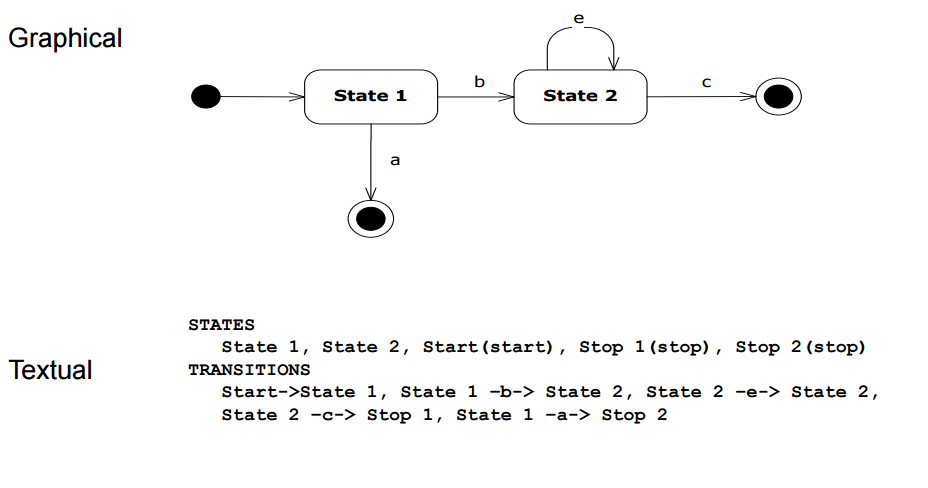
\includegraphics[width=\textwidth]{images/GraficalTextualComparison.PNG}
      \captionof{figure}{comparison between textual modeling language and graphcal modeling language for the same model}
    \end{figure}
 
%  \begin{itemize}
%  \item different approaches :  Graphical Modeling Languages, Textual Modeling Languages
%  \item 
%    \begin{figure}[ht]
%       \centering
%       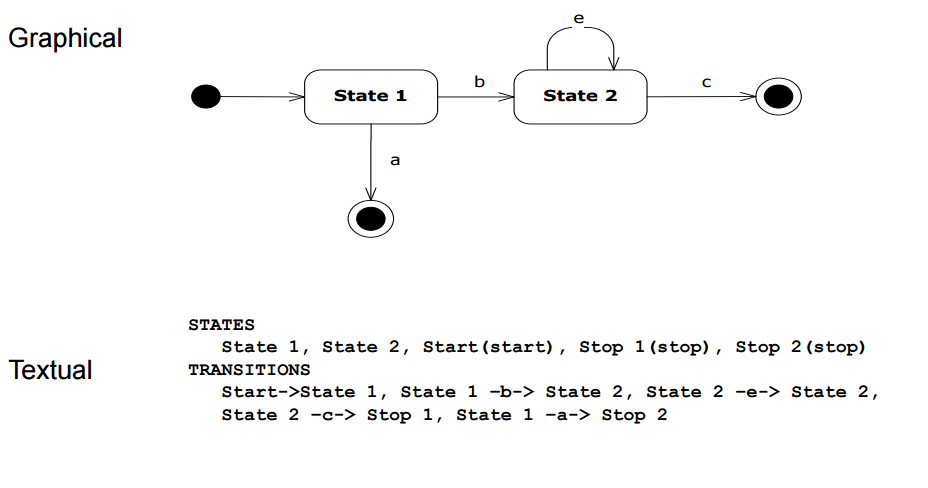
\includegraphics[width=\textwidth]{images/GraficalTextualComparison.PNG}
%       \captionof{figure}{comparison between textual modeling language and graphcal modeling language for the same model}
%     \end{figure}
%  
%  \item examples (domain experts): BPMN , SimuLink
%  \item examples (novice ): STARLOGO 
%  \end{itemize}
 
 \section{Existing Modeling Languages}
 
 \subsection{StarLogo TNG}

  \begin{itemize}
  \item is a client-based modeling and simulation software
  \item enables secondary school students and teachers to model decentralized systems through agent-based programming
  \item facilitates the creation and understanding of simulations of complex systems
  \item graphical programming blocks instead of text-based computer code
  \end{itemize}
  
  \begin{figure}[ht]
	\centering
  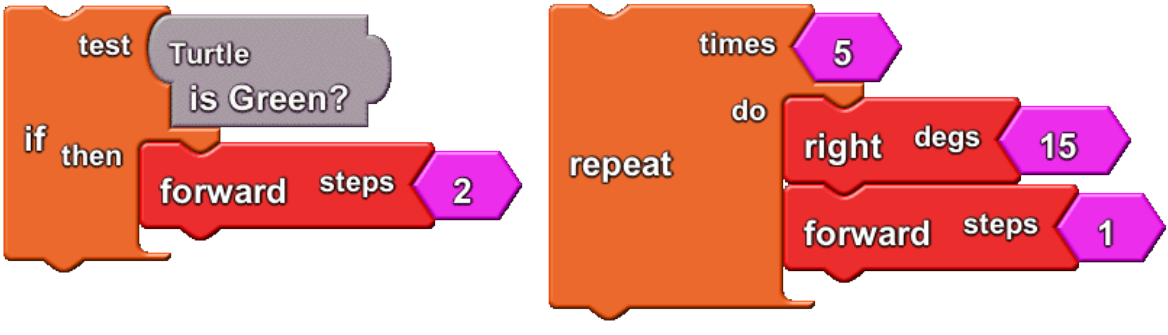
\includegraphics[width=0.5\textwidth]{images/StarLogoTNGBlocksEx.PNG}
	\caption{ StarLogo TNG’s graphical programming blocks. Example if (left) and repeat (right) blocks are shown. The
	  if block commands a Turtle agent to take two steps forward if it is green; the repeat block commands an agent to
	  repeat five times the sequence of turning right 15 degrees and taking one step forward.}
	\label{fig1}
  \end{figure}
  
   \subsection{Snatch}

  \begin{itemize}
  \item Graphical Modeling Language (similar to StarLogo)
  \item developers goal: ``make it easy for everyone,
of all ages, backgrounds, and interests, to program
their own interactive stories, games, animations, and
simulations, and share their creations with one another''
  \end{itemize}
    \begin{figure}[ht]
      \centering
      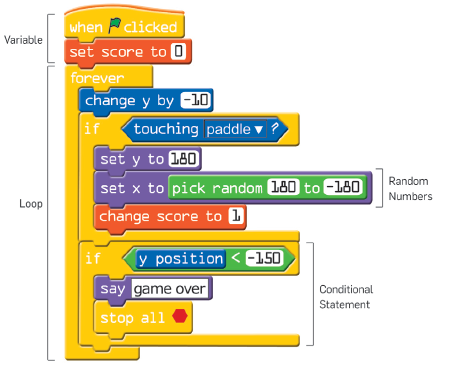
\includegraphics[width=\textwidth]{images/Snatch1.PNG}
      \captionof{figure}{Sample Scratch script (from Pong-like paddle game) highlighting computational
and mathematical concepts}
    \end{figure}
  
  
  \subsection{PhyDSL}

  \begin{itemize}
  \item textual modeling for (simple) game dev domain
  \item based on EMF
  \item allows codegeneration from the created models
  \item mobile gameplay definition sections:
    \begin{itemize}
    \item static actor definition
    \item environment and layout definition
    \item activities definition
    \item scoring rules definition
    \end{itemize}
  
  \end{itemize}
     \begin{figure}[htbp]
      \centering
      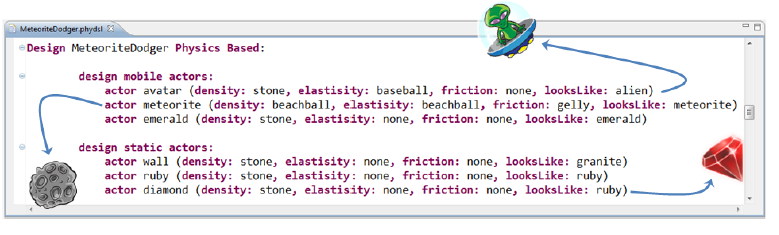
\includegraphics[width=\textwidth]{images/PhyDSL1.PNG}
      \captionof{figure}{PhyDSL: static actor definition}
    \end{figure}
       \begin{figure}[htbp]
      \centering
      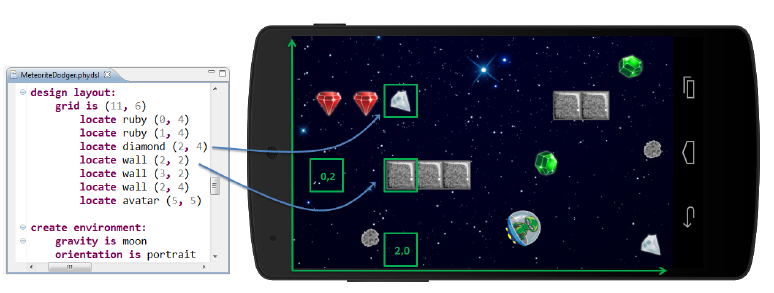
\includegraphics[width=\textwidth]{images/PhyDSL2.PNG}
      \captionof{figure}{PhyDSL: environment and layout definition}
    \end{figure}
  \begin{figure}[htbp]
      \centering
      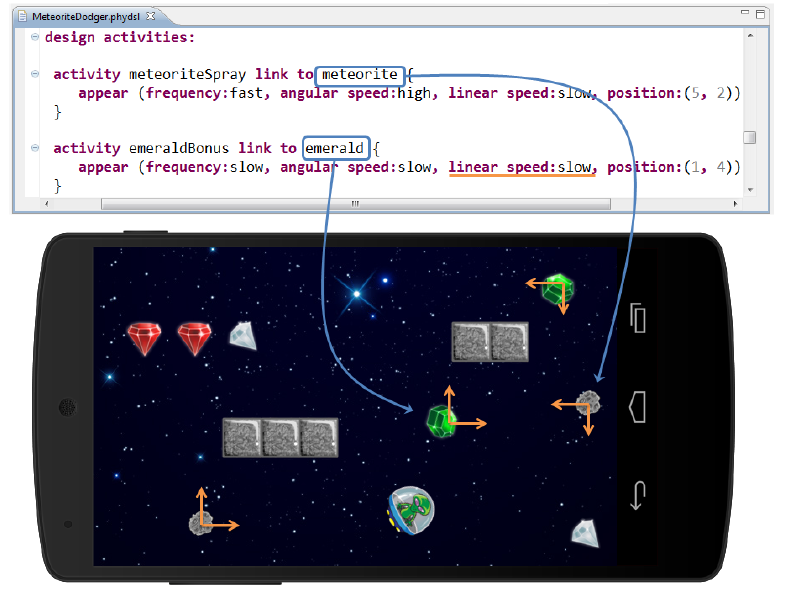
\includegraphics[width=\textwidth]{images/PhyDSL3.PNG}
      \captionof{figure}{PhyDSL: activities definition}
    \end{figure}
  
   \subsection{Lego Mindstorms}
  \begin{itemize}
  \item EV3 Programmer App or Computer Software for programming lego robots in a graphical syntax 
  \item action blocks (Green), flow blocks (Orange), sensor blocks (Yellow), data operation blocks (Red), advanced blocks (Dark blue)
  \item programms are executed on the EV3 P-brick. 
  %https://www.lego.com/en-us/mindstorms/learn-to-program
  \end{itemize}
  
  \begin{minipage}{.5\textwidth} %
	  \centering
    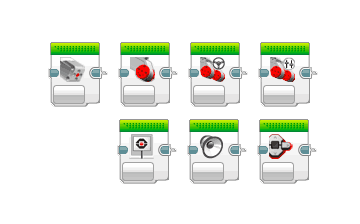
\includegraphics[width=\textwidth]{images/LearnToProgram_action_blocks_landscape.png}
	  \captionof{figure}{The action blocks control the actions of the program, e.g. motor rotations, image, sound and the light on the EV3 P-brick.}
  \end{minipage} %
  \begin{minipage}{.5\textwidth} %
	  \centering
    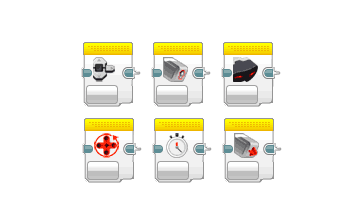
\includegraphics[width=\textwidth]{images/LearnToProgram_sensor_blocks_landscape.png}
	 \captionof{figure}{The sensor blocks allow to read the inputs e.g. from a Color sensor, IR sensor, Touch sensor.}
  \end{minipage}
  \begin{minipage}{.5\textwidth} %
	  \centering
    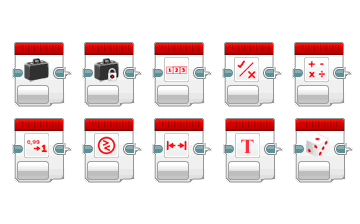
\includegraphics[width=\textwidth]{images/LearnToProgram_operations_blocks_landscape.png}
    \captionof{figure}{The data operation blocks let the user write and read variables, compare values for example.}
  \end{minipage}
  \begin{minipage}{.5\textwidth} %
	  \centering
    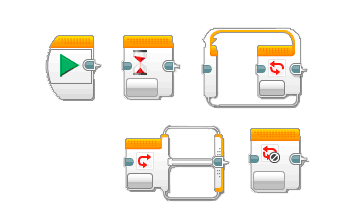
\includegraphics[width=\textwidth]{images/LearnToProgram_flow_blocks_landscape.png}
    \captionof{figure}{The Flow blocks control the flow of the program.}
  \end{minipage}
  
  
    \begin{figure}[ht]
	  \centering
    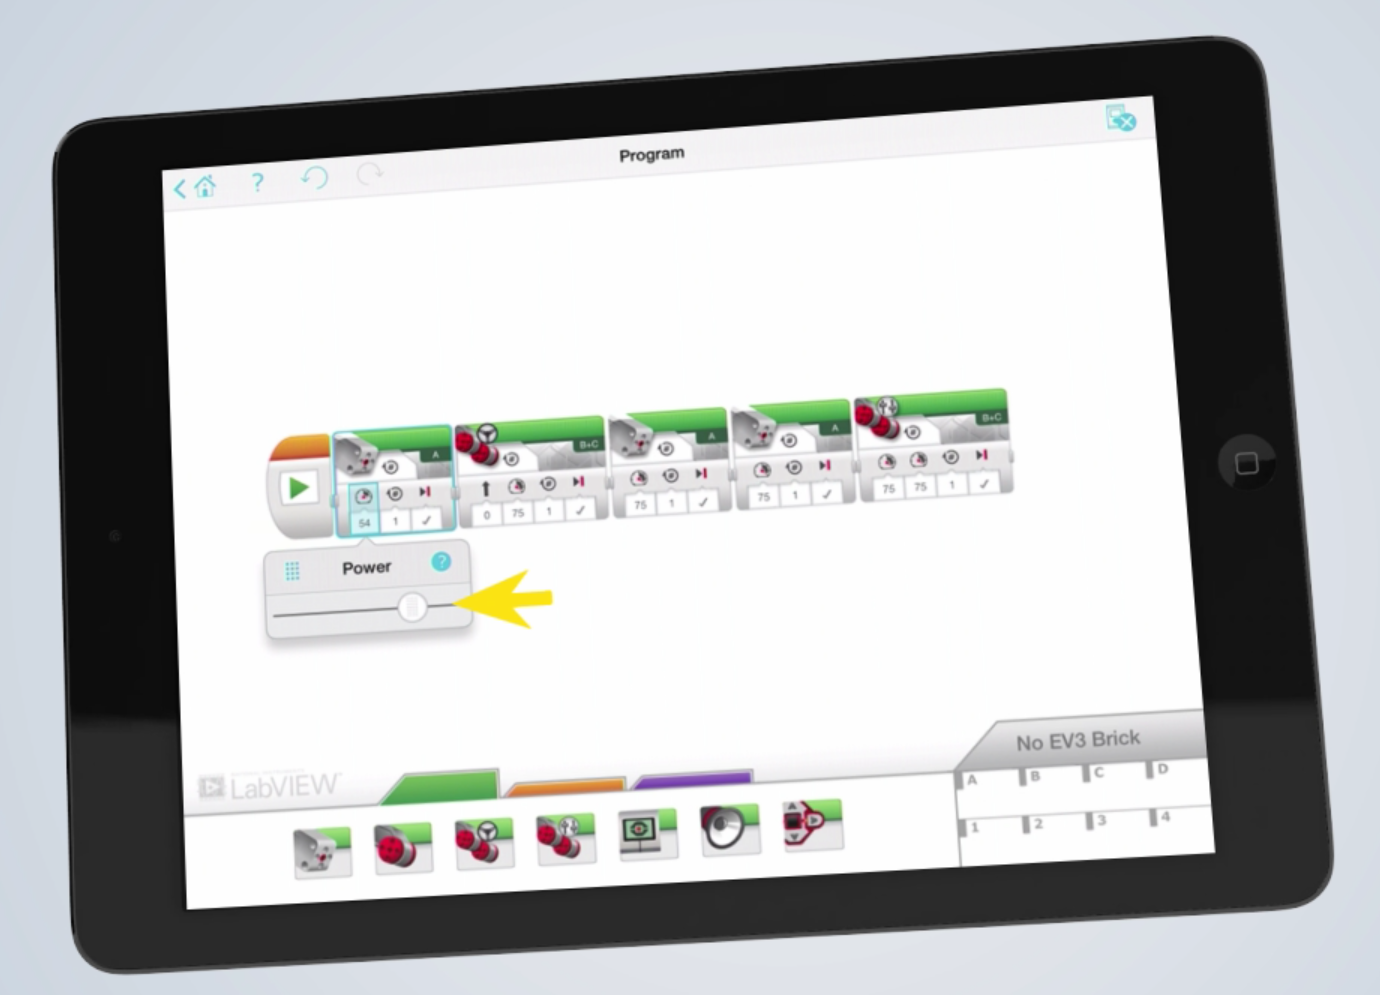
\includegraphics[width=0.5\textwidth]{images/mindstorms0.PNG}
	  \caption{EV3 Programmer App used to create programms using a graphical syntax based on blocks }
    \end{figure}

    \subsection{Sensr}
    \begin{itemize}
     \item enables people without programming skills to build mobile data collection and management tools for citizen science
    \end{itemize}

    
    \section{Creating Domain Specific Models}
    
    \subsection{Ecplise EMF}
     \subsection{Ecore}
      \begin{itemize}
	\item  a meta model  for describing models and runtime support for the models .
    \end{itemize}
    
    \subsection{Xtext}
    \begin{itemize}
      \item used to create textual DSLs for ecore (meta-)models designed in EMF
      \item syntax similar to EBNF
      \item one rule for each (meta-)model element
    \end{itemize}
    \begin{figure}[ht]
      \centering
      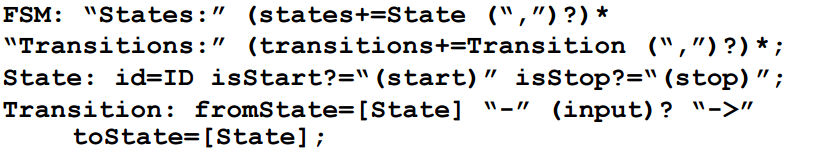
\includegraphics[width=\textwidth]{images/XTextGrammar.PNG}
      \captionof{figure}{XText Sample Grammar}
    \end{figure}
    
    \subsection{GMF}
     \begin{itemize}
     \item used to create graphcal DSLs for  models described in Ecore
     \item connects domain model and a graphical model via mapping modell
    \end{itemize}
    
    \begin{figure}[ht]
      \centering
      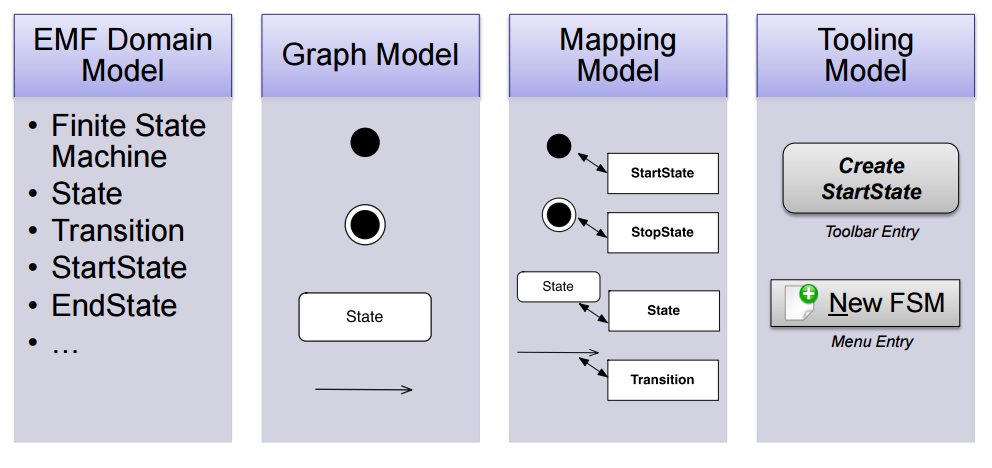
\includegraphics[width=\textwidth]{images/TableGMFSteps.PNG}
      \captionof{figure}{}
    \end{figure}

\section{Summary}\label{sec:summary}
\begin{itemize}
 \item DSM allows novices to build and explore 
their own models and learn new scientific ideas in the process
\item domain experts are supported by setting focus on domain specific problems
\end{itemize}

  
% 
% ---- Bibliography ----
% 
\nocite{*}

\bibliographystyle{splncs}
\bibliography{citations}
\end{document}

